\chapter{Results}\label{chapter:results}
\editComment{Do intro}
Following the production of the BDT discriminator shapes for data and the simulated samples and their shape systematic uncertainties described in Chapter~\refchapter:bkg}, a simultaneous fit of these shapes was performed and evaluated to measure the cross section of the signal process and its upper limit and the significance of the result.

\section{Statistical Methodology}\label{sec:statisticalModel}
The Higgs Analysis Combined Limit (\combine) tool~\cite{Combine} tool, a framework based on the RooStats package~\cite{Moneta:2010pm,Schott:2012zb}, was used to perform a binned Maximum Likelihood Fit (MLF) to evaluate measurement made using the $CL_{S}$ method~\cite{CMS-NOTE-2011-005,Khachatryan:2014jba,Cowan:2010js}.

\subsection{Likelihood Model}\label{subsec:likelihoodModel}
For the signal and background processes considered in the search, the expected event yield $\lambda$ in the bin $i$ is given by equation~\ref{eq:yields1}:

\begin{equation}
\lambda_{i} = \mu s_{i} + \sum\limits_{j} b_{j} \;
\label{eq:yields1}
\end{equation}

where $s$ and $b$ are the expected number of signal and background events and $\mu$ is the signal strength modifier.
$\mu$, as given in equation~\ref{eq:signalModifier} where $\sigma_{obs}$ is the cross section observed, is used typically to parametrise the expected signal yield in lieu of the expected cross section.
The uncertainties associated with the simulated predictions of the signal and background processes are accounted for by the inclusion of nuisance parameters $\theta$, such that $s_{i} = s_{i} (\theta)$ and $b_{i} = b_{i} (\theta)$.

\begin{equation}
\mu = \frac{\sigma_{obs}}{\sigma_{s}  \;
\label{eq:signalModifier}
\end{equation}

Assuming that the number of observed events, $n_{i}$, in any given bin will be distributed according to Poisson statistics, the probability of observing $n_{i}$ is given by equation~\ref{eq:poissonProb}.

\begin{equation}
\mathcal{P} ( n_{i} | \lambda_{i} ) = \frac{\lambda_{i}}{n_{i}!} e^{- \lambda_{i}} = \frac{ \big( \mu s_{i}(\theta) + b_{i}(\theta) \big)^{n_{i}}}{n_{i} !} e^{- \mu s_{i}(\theta) - b_{i}(\theta)}  \;
\label{eq:poissonProb}
\end{equation}

A probability density function, $\rho ( \theta | \tilde{\theta} )$ with a nominal value of $\tilde{\theta}$ for the best estimate of the nuisance, is used to describe all the sources of uncertainty for the nuisance parameters.
For the search presented in this thesis, it is assumed that each source of systematic uncertainty is either 100\% correlated or uncorrelated, thus allowing each systematic uncertainty to be incorporated into $\rho ( \theta | \tilde{\theta} )$ in a clean factorised form.
Shape uncertainties are modelled by vertically morphing the nominal shape template between between its up and down variations while the the non-prompt lepton normalisation and luminosity flat rate uncertainties are treated as log-uniform and log-normal nuisance parameters respectively~\cite{Baak:2014fta,AsymptoticFormulae}.
\combine includes the impact of the statistical uncertainty on the the aMC@NLO Z+jets sample normalisation determined in the Z+jets control region obtained as a log-normal nuisance parameter.

Therefore, the likelihood for the entire dataset can be expressed the product of the Poisson probabilities, $\mathcal{P}$, for all bins and the nuisance parameters' probability density function, as given by equation~\ref{eq:poissonLikelihood}.

\begin{equation}
\mathcal{L} ( n_{i} | \mu , \theta ) = 
\prod\limits_{i=1}^{\N} _{i} \mathcal{P} \big( n_{i} | \mu s_{i}(\theta) + b_{i}(\theta) \big) \rho ( \theta | \tilde{\theta} ) \;
\label{eq:poissonLikelihood}
\end{equation}

\subsection{$CL_{S}$ method}\label{subsec:CLsMethod}
The modified classical frequentist method, known as the $CL_{S}$ method, was used to evaluate the compatibility of data with the \emph{signal+background} (s+b) and \emph{background only} (b-only) hypotheses in terms of the siginfiance of and the limits on the signal strength measured~\cite{Cowan:2010js}.

To evaluate these hypotheses, the method constructs a test statistic, $q_{\mu}$.
The ATLAS and CMS collaborations at the LHC define $q_{\mu}$ as the log likelihood ratio for a given model with $\mu$ by equation~\ref{eq:testStatistic},

\begin{equation}
q_{\mu} =  -2 \ln \frac{ \mathcal{L}(data | \mu s , \hat{\theta_{\mu}}}{ \mathcal{L}(data | \hat{\mu} s \hat{\theta_{\mu}},  } , where 0 \leq \hat{\mu} \leq \mu \;
\label{eq:testStatistic}
\end{equation}

where $\hat{\theta_{\mu}}$ refers to the maximum likelihood estimators of $\theta$ for a given $\mu$, and 
$\hat{\mu}$ and $\hat{\theta}$ correspond to the global maximum of the likelihood. 
By definition $\hat{\mu}$ cannot take negative values as physics defines the signal rate as positive, and the constraint $\hat{\mu} < \mu$ is applied to ensure a one-sided confidence interval.

Using $q_{\mu}$, the the probability distribution functions for the \emph{s+b} and \emph{b-only} hypotheses for a given signal strength can be constructed using \emph{pseudodata} generated using toy MC.
From these probability distribution functions, the probability values for the s+b and b-only hypotheses can be defined as equations~\ref{eq:pmu} and~\ref{eq:1-pb}.

\begin{equation}
p_{\mu} = P ( q_{\mu} \geq  q_{\mu}^{obs} | \mu s + b ) = \int^{\infty}_{q_{\mu}^{obs}} f ( q_{\mu} | \mu , \theta_{\mu}^{obs} ) dq_{\mu} \;
\label{eq:pmu}
\end{equation}

\begin{equation}
1 - p_{b} = P ( q_{\mu} \geq  q_{\mu}^{obs} | b ) = \int^{\infty}_{q_{0}^{obs}} f ( q_{\mu} | 0 , \theta_{0}^{obs} ) dq_{\mu} \;
\label{eq:1-pb}
\end{equation}

The ratio of these probabilities are used to define $CL_{S} (\mu)$ in equation~\ref{eq:CLs}.

\begin{equation}
CL_{S} (\mu) = \frac{ p_{\mu} }{ 1 - p_{b} }\;
\label{eq:CLs}
\end{equation}

If for a given $\mu$, $CL_{S} < \alpha$, 
Therefore, using the upper limit for a given Confidence Limit (CL) $(1 - \alpha)$ can be given 
The  
Therefore for the 95\% CL upper limit for $\mu$ is given when $CL_{S} < 0.05$.

Therefore 

%%%%
The \emph{Asymptotic} CL$_{s}$ method was used in order to reduce computing time as the number of expected events was sufficiently large.
This method uses one representative dataset, known as the \emph{Asimov dataset}, in lieu of an ensemble of toy MC samples.
The Asimov dataset is defined as being constructed such that all observable quantities are equal to their expectation values.
A full description of this methodology is given in~\cite{Cowan:2010js}.

\section{Post-Fit Impact of the Systematic Uncertainties}\label{sec:uncertainitiesImpact}
The effect of each of the sources of systematic uncertainty following the fit is considered in terms of the pull ($\frac{ \hat{\theta} - \theta_{0} }{\Delta \theta}$) and the postfit impact of varying the sources of uncertainty by $\pm 1 \sigma$ are shown in figure~\ref{fig:systematicsPull}.

The uncertainty associated with the value of the luminosity used has the greatest impact on the 
While the JER 
The rest of the experimental uncertainties 
 
\editComment{Update shortly}
\editComment{Remark on the lumi, jer are the largest uncerts and how the rest of the experimental uncerts are considerably smaller}

\begin{figure}[htbp]
\begin{center}
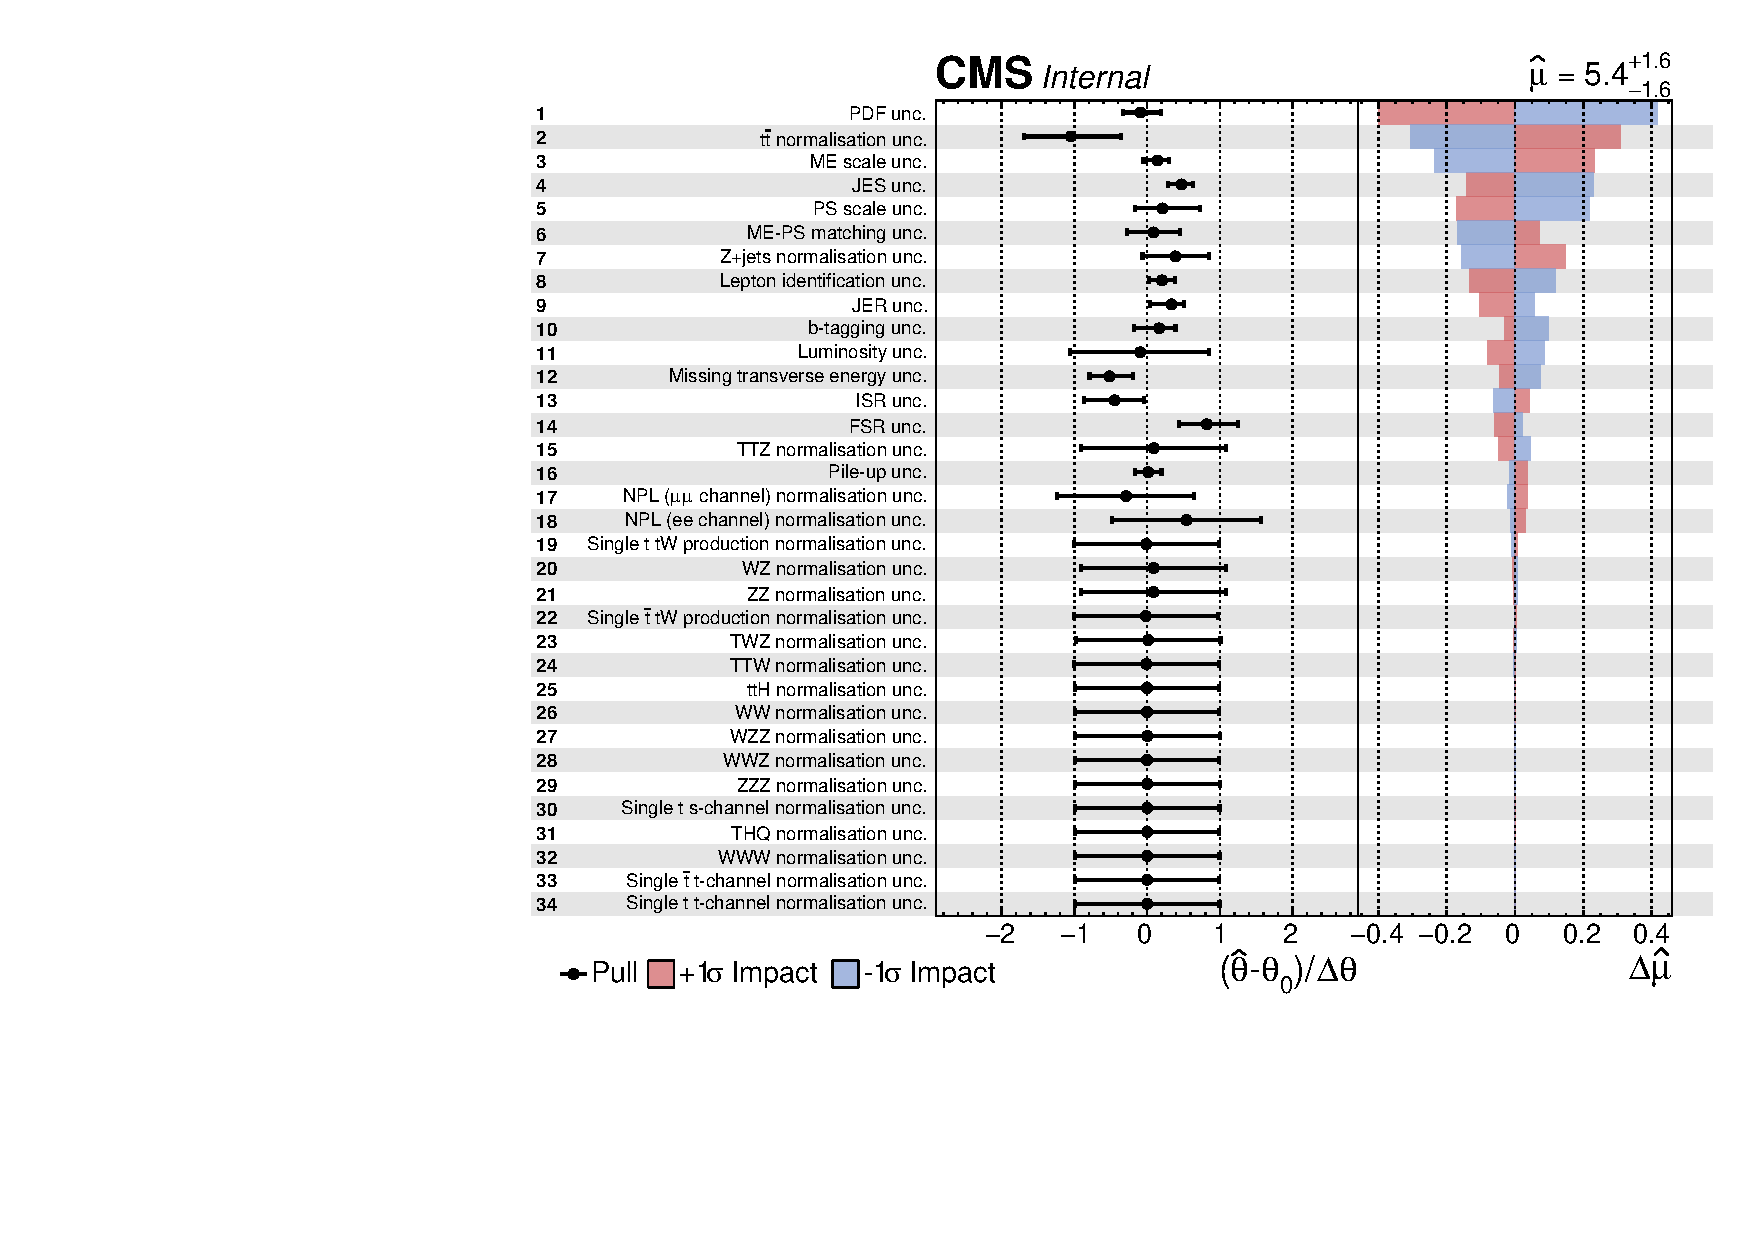
\includegraphics[width=0.97\textwidth]{figs/results/systematicsImpact.pdf}
\caption{The impact of each of the systematic uncertainties considered on the measurement made.}
\label{fig:systematicsPull}
\end{center}
\end{figure}

\section{Statistical Analysis Results}
\editComment{UPDATE BEFORE SUBMISSION}
For the combination of both of the final states, at the 95\% CL, the cross section for tZq production was measured to be $X^{+Y}_{-Z}$, which is within the uncertainties of the SM prediction.
This result corresponds to an observed significance of $X_{-Z}^{+Y} \sigma$ against an expected significance of $X_{-Z}^{+Y} \sigma$, which is in agreement with the SM cross section of  $0.0758^{+Y}_{-Z} \pb$.

The observed signal strengths, measured cross sections, and corresponding significances for the individual channels and their combination are shown in full in table~\ref{tab:shapetxs}.

\begin{table}[!h]
   \centering
   \caption{The observed signal strengths and corresponding cross sections for
   the individual channels and the channels combined at the 95\% CL.}
   \begin{tabular}{cccc}
       \hline
       Channel & $ee$ & $\mu\mu$ & \textbf{Combination} \\
        \hline
       Signal strength (expected) & $1_{-1.58716}^{+1.63708}$ & $X_{-0.606435}^{+0.663951}$ & $X_{-0.56704}^{+0.613355}$ \\
       Cross section (fb) & $X_{-Z}^{+Y}$ & $X_{-Z}^{+Y}$ & $X_{-Z}^{+Y}$ \\
       Significance (expected) ($\sigma$) & $0.628127_{-Z}^{+Y}$ & $1.66857_{-Z}^{+Y}$ & $1.78824_{-Z}^{+Y}$ \\
       Significance (observed) ($\sigma$) & $X_{-Z}^{+Y}$ & $X_{-Z}^{+Y}$ & $X_{-Z}^{+Y}$ \\
    \end{tabular}
   \label{tab:shapetxs}
\end{table}

At the time of writing this thesis, discussions were being undertaken on how best to take this search forward.
The two options under consideration were presenting it as a standalone search or a combination with the trilepton search following the inclusion of data collected by the CMS detector during 2017.
As such, while the result presented here is not a final result, an updated result is intended presented in a future CMS publication in the near future.

\section{Discussion of other searches for tZq at the Large Hadron Collider}
The search for the dilepton final state of a singly produced top in association with a Z boson presented in this thesis is the first one that has been undertaken at the LHC.
As such while these results cannot be compared against any previous or competing results, searches for tZq have been made for the trilepton final state at $\sqrt{s} = 8 \TeV and 13 \Tev$.

Following the trilepton tZq search at $\sqrt{s} = 8 \TeV$ by the CMS collaboration which reported a significance of 2.9 standard deviations ~\cite{Sirunyan:2017kkr}, at $\sqrt{s} = 13 \TeV$ both the ATLAS and CMS collaborations  have reported significances in excess of 3.0 standard deviations, 4.2 and 3.7 respectively~\cite{Aaboud:2017ylb,Sirunyan:2017nbr}.
Despite the dilepton final state having a larger production cross section than the fully leptonic final state, the similarity of the final state topology to those of significantly larger backgrounds limits the ability to observe it.

Therefore, as the search  is currently statistically limited, it is anticipated that including data collected by the CMS experiment during 2017 could allow for a significance close to or in excess of 3.0 standard deviations to be observed.
Even if additional statistics isn't sufficient for an observation to be made of the dilepton final state, when combined with the trilepton final state result it should be possible to measure the process with a 5.0 standard deviations significance.
